\chapter{Basic Topology}
  \label{chapter:Basic Topology}
    \section{Quick recap on Sets, Maps, and Equivalence classes}
      \subsection*{Set theory}
        A set is a well-defined collection of objects. The cardinality of a
        set $A$, denoted as $|A$, is the number of elements in the set. The
        elements in a set are unique, and the ordering of elements in a set
        doesn't matter. The set with no elements at all is known as the null
        set, denoted as $\phi$ or $\{\}$. Given a set $A$, we also have $A^c$
        as another set that contains all other elements that are not in $A$.
        $A^c$ is known as "$A$ complement".

        Given two sets $A$ and $B$, we can produce new sets from $A$ and $B$
        using the following operations \[\cap \quad \cup \quad \backslash \]
        known as the intersection, the union and the complement respectively.
        \begin{enumerate}
          \item{$A\cap B$: is a new set that contains elements that are in
          both $A$ and $B$.}
          \item{$A\cup B$: is a new set that contains elements that are in
          either $A$ or $B$.}
          \item{$A \backslash B$: is a new set that contains elements that
          are in $A$ but not in $B$. The complement is also sometimes written
          as $A - B$.}
        \end{enumerate}
        These operations obey De Morgan's laws. The two more important ones
        are: $(A \cup B)^c = A^c \cap B^c$ and $(A \cap B)^c = A^c \cup B^c$.
        There is also a very important theorem known as the
        "inclusion-exclusion" principle, which is only stated in name here
        but can be found in any introductory mathematics books.

        Suppose we have two sets $A$ and $B$. If $\forall b \in B,\, b \in
        A$, we say that $B \subset A$, or that $B$ is a subset of $A$. For a
        set $A$, the set of all its subsets is known as the power set of $A$,
        denoted as $\mathcal{P}(A)$. E.g, if $A = \{1,2,3\}$, then
        $\mathcal{P}(A) =$ $\{ \{\}, \{1\}, \{2\}, \{3\}, \{1,2\},
        \{2,3\},\{1,3\},\{1,2,3\}\}$. We can easily prove that
        $|\mathcal{P}(A)|=2^{|A|}$.

        Two sets $A$ and $B$ are defined to be equal if $A \subset B$ and $B \subset A$.

        Relationships between sets can be illustrated very easily by a Venn
        diagram, as shown in Figure~\ref{fig: set relations}.
        \begin{figure}
          \centering
          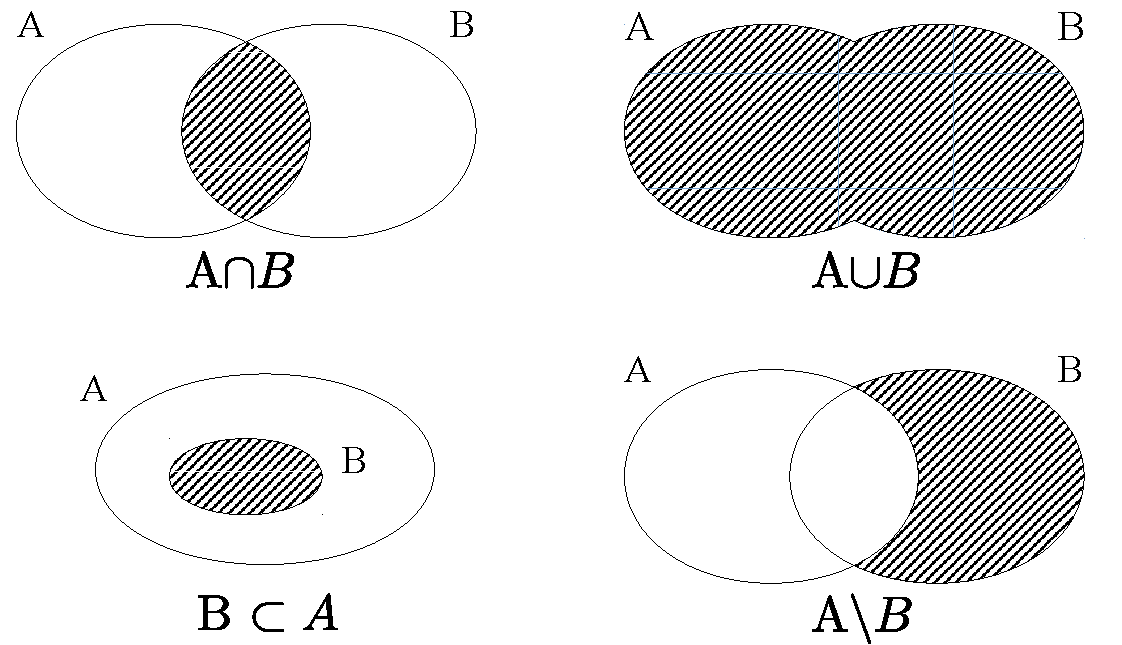
\includegraphics[width=0.7\textwidth, trim={0cm 0cm 0cm
          0cm},clip]{setRelations}
          \caption[]{}
          \label{fig: set relations}
        \end{figure}
      \subsection*{Maps}
        \begin{definition}[Maps between sets]
          Let $A$ and $B$ be two sets. A map $f$ is a many-to-one or
          one-to-one relation between elements in set $A$ and elements in set
          $B$. I.e, $\forall a \in A$, we have a corresponding element $f(a)
          \in B$. We denote a map in one of these two ways:
          \[A \xrightarrow{f} B \quad \quad f: A \rightarrow B\]
        \end{definition}
        \begin{definition}[Images and pre-images]
          Suppose we have $f: A\rightarrow B$. We say that $f(A)$ is the
          image of $A$ under $f$.\\
          We can also define a concept known as the pre-image of a map $f$,
          which we denote as $f^{-1}$. I.e, $\forall b \in B$, we have:
          $f^{-1}(b) = \{a \in A \,|f(a) = b\}$. Note that $f^{-1}$ is not necessarily a map, because $f^{-1}$ can be one-to-many.
        \end{definition}
        \begin{definition}(Injective, Surjective and Bijective)
          \begin{itemize}
            \item{A map $f: A \rightarrow B$ is one-to-one, or injective, if
            $\forall a,b \in A$, $f(a) = f(b) \Leftrightarrow a=b$.}
            \item{A map $f: A \rightarrow B$ is onto, or surjective, if
            $\forall b \in B$, $\exists a \in A$ such that $f(a) = b$. In other words, $f(A) = B$.}
            \item{A map $f: A \rightarrow B$ is bijective if and only if it is both surjective and injective.}
          \end{itemize}
        \end{definition}
        \textcolor{red}{More to come! In progress!}